\section{System Models and Terms}   \label{chap:systemModel}

This chapter will cover common terms for describing computation, timing, and analysis in the context of real-time systems.
Note that chapter-specific terms and notation (for example, engine control tasks) will be covered in the relevant chapter.

\subsection{Modeling Basic Computation: Jobs and Tasks}

% \textit{Jobs} and \textit{tasks} are two tools used to characterize demand and help perform schedulability analysis.

\subsubsection{Jobs}

A job, $j_i$, is the smallest unit for modeling real-time computation characterized by the tuple $j = (a,e,d)$ where $a$ is the release time, $d$ is the relative deadline, and $e$ is the execution time.
The release time, $a$, is the earliest time at which processor time may be allocated to the job.
The relative deadline, $d$, is the time by which $e$ units of processor time must be allocated to the job to avoid a \textit{deadline miss}.
In the context of the airbag ECU, a \textit{deadline miss} is when the ECU calculation is not completed early enough to signal the airbag for deployment and the passenger collides with the steering wheel or dashboard. 
The execution time, $e$, is the amount of processor time required to complete the requested computation. 
Figure \ref{fig:rt-job} illustrates a single job and its typical parameters.

\begin{figure}[!htbp]
    \centering
    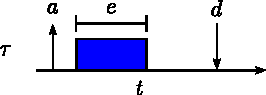
\includegraphics[width=0.50\linewidth]{fig/singleJob.pdf}
    \caption{Real-Time Job Parameters} A single job of task $\tau$ with release time $a$, execution time $e$, and deadline $d$.
    The x-axis is time where an upward arrow indicates the release of a job and a downward arrow represents the deadline of the job.
    The box represents execution time allocated to task $\tau$.
    \label{fig:rt-job}
\end{figure}

\subsubsection{Task}

A task, $\tau_i$, is an infinite series of jobs characterized by the tuple $\tau_i = (a,p,c,d)$ where $a$ is the offset of the task,
$p$ is either the period or minimum interarrival time,
$c$ is the WCET,
and $d$ is the relative deadline.
The offset, $a$, is the time after $t=0$ at which the first job of the task is released.
Tasks may be either \textit{aperiodic} (also known as \textit{sporadic}) or \textit{periodic}.
Sporadic tasks release jobs at irregular intervals.
If $\tau$ is a sporadic task, $p$ represents the minimum interarrival time between successive jobs.
Periodic tasks release jobs at regular intervals.
If $\tau$ is a periodic task, $p$ represents the fixed interarrival time between successive jobs.
The WCET, $c$, is the upper bound on execution time for all jobs the task may release.
The relative deadline, $d$, is the relative deadline for all jobs of the task such that a job released at time $t$ is has a deadline at time $t+d$.
Figure \ref{fig:rt-task} illustrates a two tasks, one sporadic and one periodic, and their typical parameters.

\begin{figure}[!htbp]
    \centering
    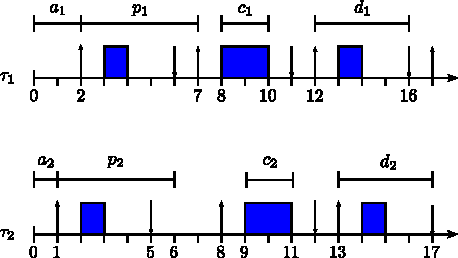
\includegraphics[width=0.75\linewidth]{fig/taskParameters.pdf}
    \caption{Real-Time Task Parameters: Periodic and Sporadic}
    Task $\tau_1 = (a_1=2, p_1 = 5, c_1=2, d_1=4)$ is a periodic task.\\
    Task $\tau_2 = (a_2=1,p_2=5,c_2=2,d_2=4)$ is an aperiodic task.\\
    Note that $\tau_1$, being periodic, has fixed releases $p_1$ units of time apart whereas $\tau_2$, being aperiodic, has releases \textit{at least} $p_2$ units apart.
    \label{fig:rt-task}
\end{figure}

\subsubsection{Task Set}

When more than one task is needed to describe all computational loads, tasks are represented by a task set, $\Tau = \{\tau_1, \tau_2, \dots, \tau_n\}$, a collection of individual tasks.
From this task set, an additional parameter, the hyperperiod $H$, can be derived.
The hyperperiod $H$ represents the least common multiple (LCM) of all periods (or minimum interarrival times) in  the task set.
Formally, $H = \text{LCM}(p_1, p_2, \dots, p_n)$.
This hyperperiod represents when the pattern of computation repeats.

\subsection{Characterizing Demand}

With some fundamental tools for modeling computation covered, we now describe methods of representing the total computation a task (or set of tasks) may require. 

\subsubsection{Utilization}

One such method is utilization, the ratio of WCET to period.
For an individual task, $\tau_i$, utilization is given by:
\begin{equation}
    u_i = \frac{c_i}{p_i}.
\end{equation}
The utilization for a task set is then,
\begin{equation}
    U = \sum_{i \in \Tau} \frac{c_i}{p_i}.
\end{equation}

Note that while utilization describes the ratio of time consumed to time available, it does not describe the change in computational load over time.

\subsubsection{Demand and the Demand Bound Function}

To provide a more precise representation of computation over time, \textit{demand} is used.
The \textit{demand} over some time interval $[t_1,t_2]$ is the sum of all WCETs of jobs with release time and deadline in the interval.
Figure \ref{fig:rt-demand} illustrates how tasks contribute to demand.
Demand, however, only reflects a particular interval of time and not any possible interval.
To address demand over any interval, the Demand Bound Function (DBF) was introduced by Baruah et al. \cite{baruah_preemptively_1990}.
The DBF is a function which characterizes demand by providing the maximum cumulative execution time a set of tasks may require from a processor over any interval of size $\delta$. 
The formal definition presented in Baruah et al. \cite{baruah_preemptively_1990} is used here.
\begin{definition}[Demand bound Function]\label{def:dbf}
    The \textit{demand bound function}, $DBF(\tau,\delta)$, gives the cumulative WCET of all jobs of $\tau$ with both release times and deadlines within any time interval of length $\delta$.
\end{definition}
Note that since the DBF describes demand over any interval, the DBF is typically more complex to calculate than utilization.

\begin{figure}[!htbp]
    \centering
    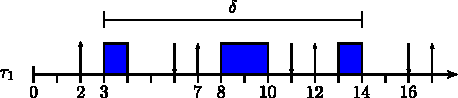
\includegraphics[width=0.75\linewidth]{fig/demandExample.pdf}
    \caption{Real-Time Demand Example}
    Task $\tau_1 = (a_1=2, p_1 = 5, c_1=2, d_1=4)$ is a periodic task.\\
    The \textit{demand} over interval $\delta = [3,14]$ is $2$.
    Since first job's release at time $t=2$ is not in the interval, the WCET of the first job is not counted towards demand.
    The second job's release time and deadline are in the interval so the WCET of the second job counts towards demand.
    The third job deadline at time $t=16$ is not in the interval and thus the WCET of the third job is not counted towards the demand.
    \label{fig:rt-demand}
\end{figure}

\subsection{Feasibility and Schedulability}

With utilization and the DBF as tools for modeling computation, our aim is to determine whether computation can be performed without missing deadlines.
To do so requires generating a schedule that ensures every job of every task is allocated the appropriate processor time to complete its execution before its deadline.
The first step in this process is feasibility analysis.

\subsubsection{Schedules}

To place feasibility and schedulability in context, we first examine schedules.
A \textit{schedule} is an assignment of tasks to a processor (or set of processors) which represents when (and thus, for how long) each job and task is executed.
Formally, a schedule for a single processor is a function which can be given as:
\begin{equation}
    \sigma(t) = i \; | \; t \in \mathbb{R}^+, \; i \in \mathbb{Z}
\end{equation}
where $t$ represents time and $i$ represents the index of the task being executed where index zero is no task (the processor is idle).
Figure \ref{fig:rt-schedule} gives a simple schedule for two tasks.

\begin{figure}[!htbp]
    \centering
    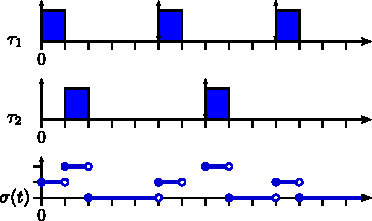
\includegraphics[width=0.5\linewidth]{fig/scheduleExample.pdf}
    \caption{Real-Time Demand Example}
    Task $\tau_1 = (a_1 = 0, p_1 = 5, c_1 = 1, d_1 = 5)$ and is periodic.\\
    Task $\tau_2 = (a_2 = 0, p_2 = 7, c_2 = 1, d_2 = 7)$ and is also periodic.\\
    Note the value of $\sigma(t)$ indicates which task is to be executing\\
    where $\sigma(t) = 0$ indicates no task is scheduled to run.
    \label{fig:rt-schedule}
\end{figure}

Given a set of tasks and processors to execute the tasks on, we now turn our attention to whether any schedule can be made, a process known feasibility analysis, and whether a particular scheduling algorithm algorithm could make a feasible schedule, a process known as schedulability analysis.

\subsubsection{Feasibility Analysis}

As mentioned above, feasibility analysis in a real-time system is the process of determining whether there exists \textit{any} schedule which could guarantee all tasks meet their deadlines.
Using utilization, a simple feasibility result for single processors where tasks are preemptible (they may be interrupted at any time to switch to another task) comes from Liu and Leyland \cite{liu_scheduling_1973}.
If utilization is less than one ($U \leq 1$) than the total time required by tasks is less than the processor availability.

Using the DBF, feasibility may be checked by checking whether the demand over any interval of length $\delta$ exceeds processor availability. CITE
For example, in the case of a single processor where tasks are preemptible the following must hold:
\begin{equation}
    \dbf(\tau,\delta) \leq \delta \; \forall \; \delta \in \mathbb{R}^+
\end{equation}
In short, if the demand of a set of tasks over an interval is greater than the size of the interval itself then it is impossible to schedule on a single processor.

Note that the results described above only apply to single processors where tasks may be interrupted at any time.
Other feasibility results exist for different scheduling settings such as nonpreemptive tasks CITE, multiple processors CITE, precedence constraints CITE, or a combination thereof.
Additionaly complications exists for systems where computation is performed on heterogeneous architectures CITE (processors with different speeds, for example) or where certain tasks must be completed by specific processors (as opposed to any processor) CITE. 
However, we will not cover those results here as our focus is on changing core real-time parameters.

While feasibility is a necessary condition of a real-time system with temporal guarantees, feasibility does not prescribe a particular schedule to satisfy each task's computation requirement.
To effectively schedule the tasks, schedulability analysis is used.

\subsubsection{Schedulability}

There are many algorithms for creating schedules for a set of tasks.
In general, scheduling algorithms determine which task or job should run by assigning priorities.
\textit{Fixed priority algorithms} assign each task a fixed priority.
Under fixed priority algorithms, the task with the highest priority that has a job released but not executed is scheduled to run.
Only after the highest priority task's active job is completed may the next-hightest task's job run.
\textit{Dynamic priority algorithms} allow the priorities of tasks to change in time.
Although dynamic priority scheduling algorithms honor the same heirarchy as fixed priority algorithms (meaning the task with the highest priority that has a job released but not executed is scheduled to run before others), task priorities may change during operation which prompts the processor to abandon the former highest-priority task in favor of the newest highest-priority task.

As with feasibility analysis, the algorithms used differ depending on properties of the processors and task such as preemptibility, the number of properties, and whether precedence constraints exist.
In any case, we may examine two simple scheduling algorithms for preemptive tasks on a single processor: Earliest Deadline First (EDF), a dynamic priority algorithm, and Rate Monotonic (RM), a fixed priority algorithm.

EDF assigns the highest priority to tasks with the earliest deadline and lowest priority to latest deadline.
Under preemptive scheduling, this requires interrupting executing tasks if a task with an earlier deadline has a job ready to execute.
Since the task with the earliest deadline will frequently change as time passes, tasks frequency trade priorities.
In the context of preemptive tasks on a uniprocessor, the schedulability test for EDF is identical to the aforementioned feasibility test: $U \leq 1$.

In contrast, RM assignes the highest priority to tasks with the smallest period and lowest priority to the largest period.
Since task periods are traditionally fixed, the priorities will not change as time passes.
In the context of preemptive tasks on a uniprocessor, a sufficient schedulability test for RM is given by Liu and Leyland \cite{liu_scheduling_1973}:
\begin{equation}
    U \leq n \cdot (n^{\frac{1}{n}}-1)
\end{equation}
where $n$ is the number of tasks.
Note that a task set which does not meet the criteria above is may still be schedulable by RM but requires additional analysis beyond utilization.

Here, we also highlight a key distinction between feasibility and schedulability.
Task sets which are feasible by \textit{any} schedule may not be schedulable by a particular algorithm.
Consider the task set $\Tau = {\tau_1, \tau_2}$ where $\tau_1 = (0,2,1,2)$ and $\tau_2 = (0,7,3.3,7)$.
The utilizations are $u_1 = 0.5$ and $u_2 = 0.47$.
By the utilization feasibility test, there exists a schedule where neither task misses a deadline.
Figure \ref{fig:rmNotSchedulable}, however, shows how RM cannot schedule the two tasks without missing a deadline.
In contrast, Figure \ref{fig:edfSchedulable} shows how EDF can schedule the two tasks without missing a deadline.

\begin{figure}[!htbp]
    \centering
    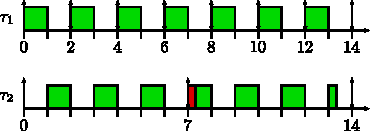
\includegraphics[width=0.75\linewidth]{fig/rmNotSchedulable.pdf}
    \caption{Rate Monotonic Missing a Deadline}
    Task $\tau_1 = (0,2,1,2)$ and is periodic.\\
    Task $\tau_2 = (0,7,3.3,7)$ and is also periodic.\\
    Note that at time $t=6$ under RM, $\tau_1$ is the highest priority.
    This prevents $\tau_2$ from completing the last $0.3$ units of execution before its deadline at $t=7$.
    The remaining $0.3$ units executed at and after $t=7$ are highlighted in red, illustrating the deadline miss.
    \label{fig:rmNotSchedulable}
\end{figure}

\begin{figure}[!htbp]
    \centering
    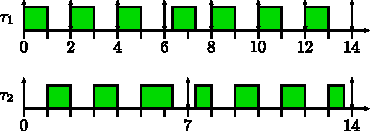
\includegraphics[width=0.75\linewidth]{fig/edfSchedulable.pdf}
    \caption{Earliest Deadline First Making Deadlines}
    Task $\tau_1 = (0,2,1,2)$ and is periodic.\\
    Task $\tau_2 = (0,7,3.3,7)$ and is also periodic.\\
    Note that unlike RM, at time $t=6$ EDF maintains $\tau_2$ as the highest priority since its next deadline is earlier than $\tau_1$'s deadline.
    The initial execution of $\tau_1$'s fourth job is slightly delayed but still finishes before its deadline.
    \label{fig:edfSchedulable}
\end{figure}

\subsection{System Model Summary}

To summarize the system model, we've covered how \textit{jobs} and \textit{tasks} are used to describe individual real-time computational workloads.
\textit{Utilization} and \textit{demand} are then used to describe the computational requirements of a set of tasks.
Together, these help system designers perform \textit{feasibility} and \textit{schedulability} analysis to determine whether a \textit{schedule} exists that guarantees temporal correctness and, if so, which scheduling algorithms could schedule the tasks.

\subsection{Integrating Real-Time Systems with Physical Dynamics}

To illustrate how tying physical dynamics brings complexity to real-time systems, consider the typical sporadic task definition: $\tau = (a,p,c,d)$.
In the examples above, these parameters are assumed to be fixed.
Suppose, however, that the real-time task cannot have a fixed minimum interarrival time, $p$.
Instead, suppose $p$ is a function of some physical dynamic modeled as $x(t)$, a variable which changes over time.
To properly determine utilization or demand, we may, for example, need to understand minimum and maximum values of $x(t)$ as well as upper and lower bounds on $\dot{x}$ and $\ddot{x}$.
Even with the appropriate model for $x(t)$, we now need to calculate utilization or demand using a variable interarrival time.
Without a utilization bound or DBF, we cannot perform feasibility or schedulability analysis.

In the following chapters, we will examine how real-time tasks used for short circuit detection and spark ignition in internal combustion engines connect real-time tasks to physical dynamics.
We will explore how bounds on the changing physical dynamics are then used to simplify feasibility and schedulability analysis.